\subsection{Konzeptvalidierung}
\label{subsec:Konzeptvalidierung}

\subsubsection{Validierung der Hardware}
\label{subsubsec:HW_Val}
Die Validierung der Hardware ist ein wichtiger Schritt um Denk- und Designfehler zu entdecken bzw. den geplanten Betrieb der Hardware sicherzustellen. Aus diesem Grund wird in diesem Unterkapitel die Validierung der Hardware thematisiert und mit Abbildungen anschaulich dargestellt. Bevor jedoch die Validierung von statten geht, werden die verwendeten Gerätschaften im nächsten Abschnitt kurz erläutert.\\
\paragraph{\textbf{Verwendete Gerätschaften}}[0.4cm]
{\begin{minipage}[b][9cm][t]{0.42\textwidth}
Damit die Hardware validiert werden kann, braucht es spezielle Geräte. Zum einen wird ein FLUKE 117 (Abbildung \ref{fig:FLUKE}), ein handliches RMS Multimeter, benutzt. Zwei Hauptfunktionen des FLUKEs werden hauptsächlich verwendet, diese sind das Messen von Gleichspannung, sowie die Messgerätfunktion Kontinuität, um zu testen ob elektrische Verbindungen bestehen \cite{FLUKE}. Zum anderen wird der TDS 210, ein Digitales Real-Time Oszilloskop von Tektronix, verwendet, um Spannungsverläufe zu analysieren. In Abbildung \ref{fig:KO} ist dieser zu sehen. Um genaue Eingangsspannungen generieren zu können, wird ein Speisegerät verwendet, welches in der Abbildung \ref{fig:PowerSupply} zu sehen ist.
\end{minipage}}
{\begin{minipage}[b][9cm][t]{0.57\textwidth}
\centering
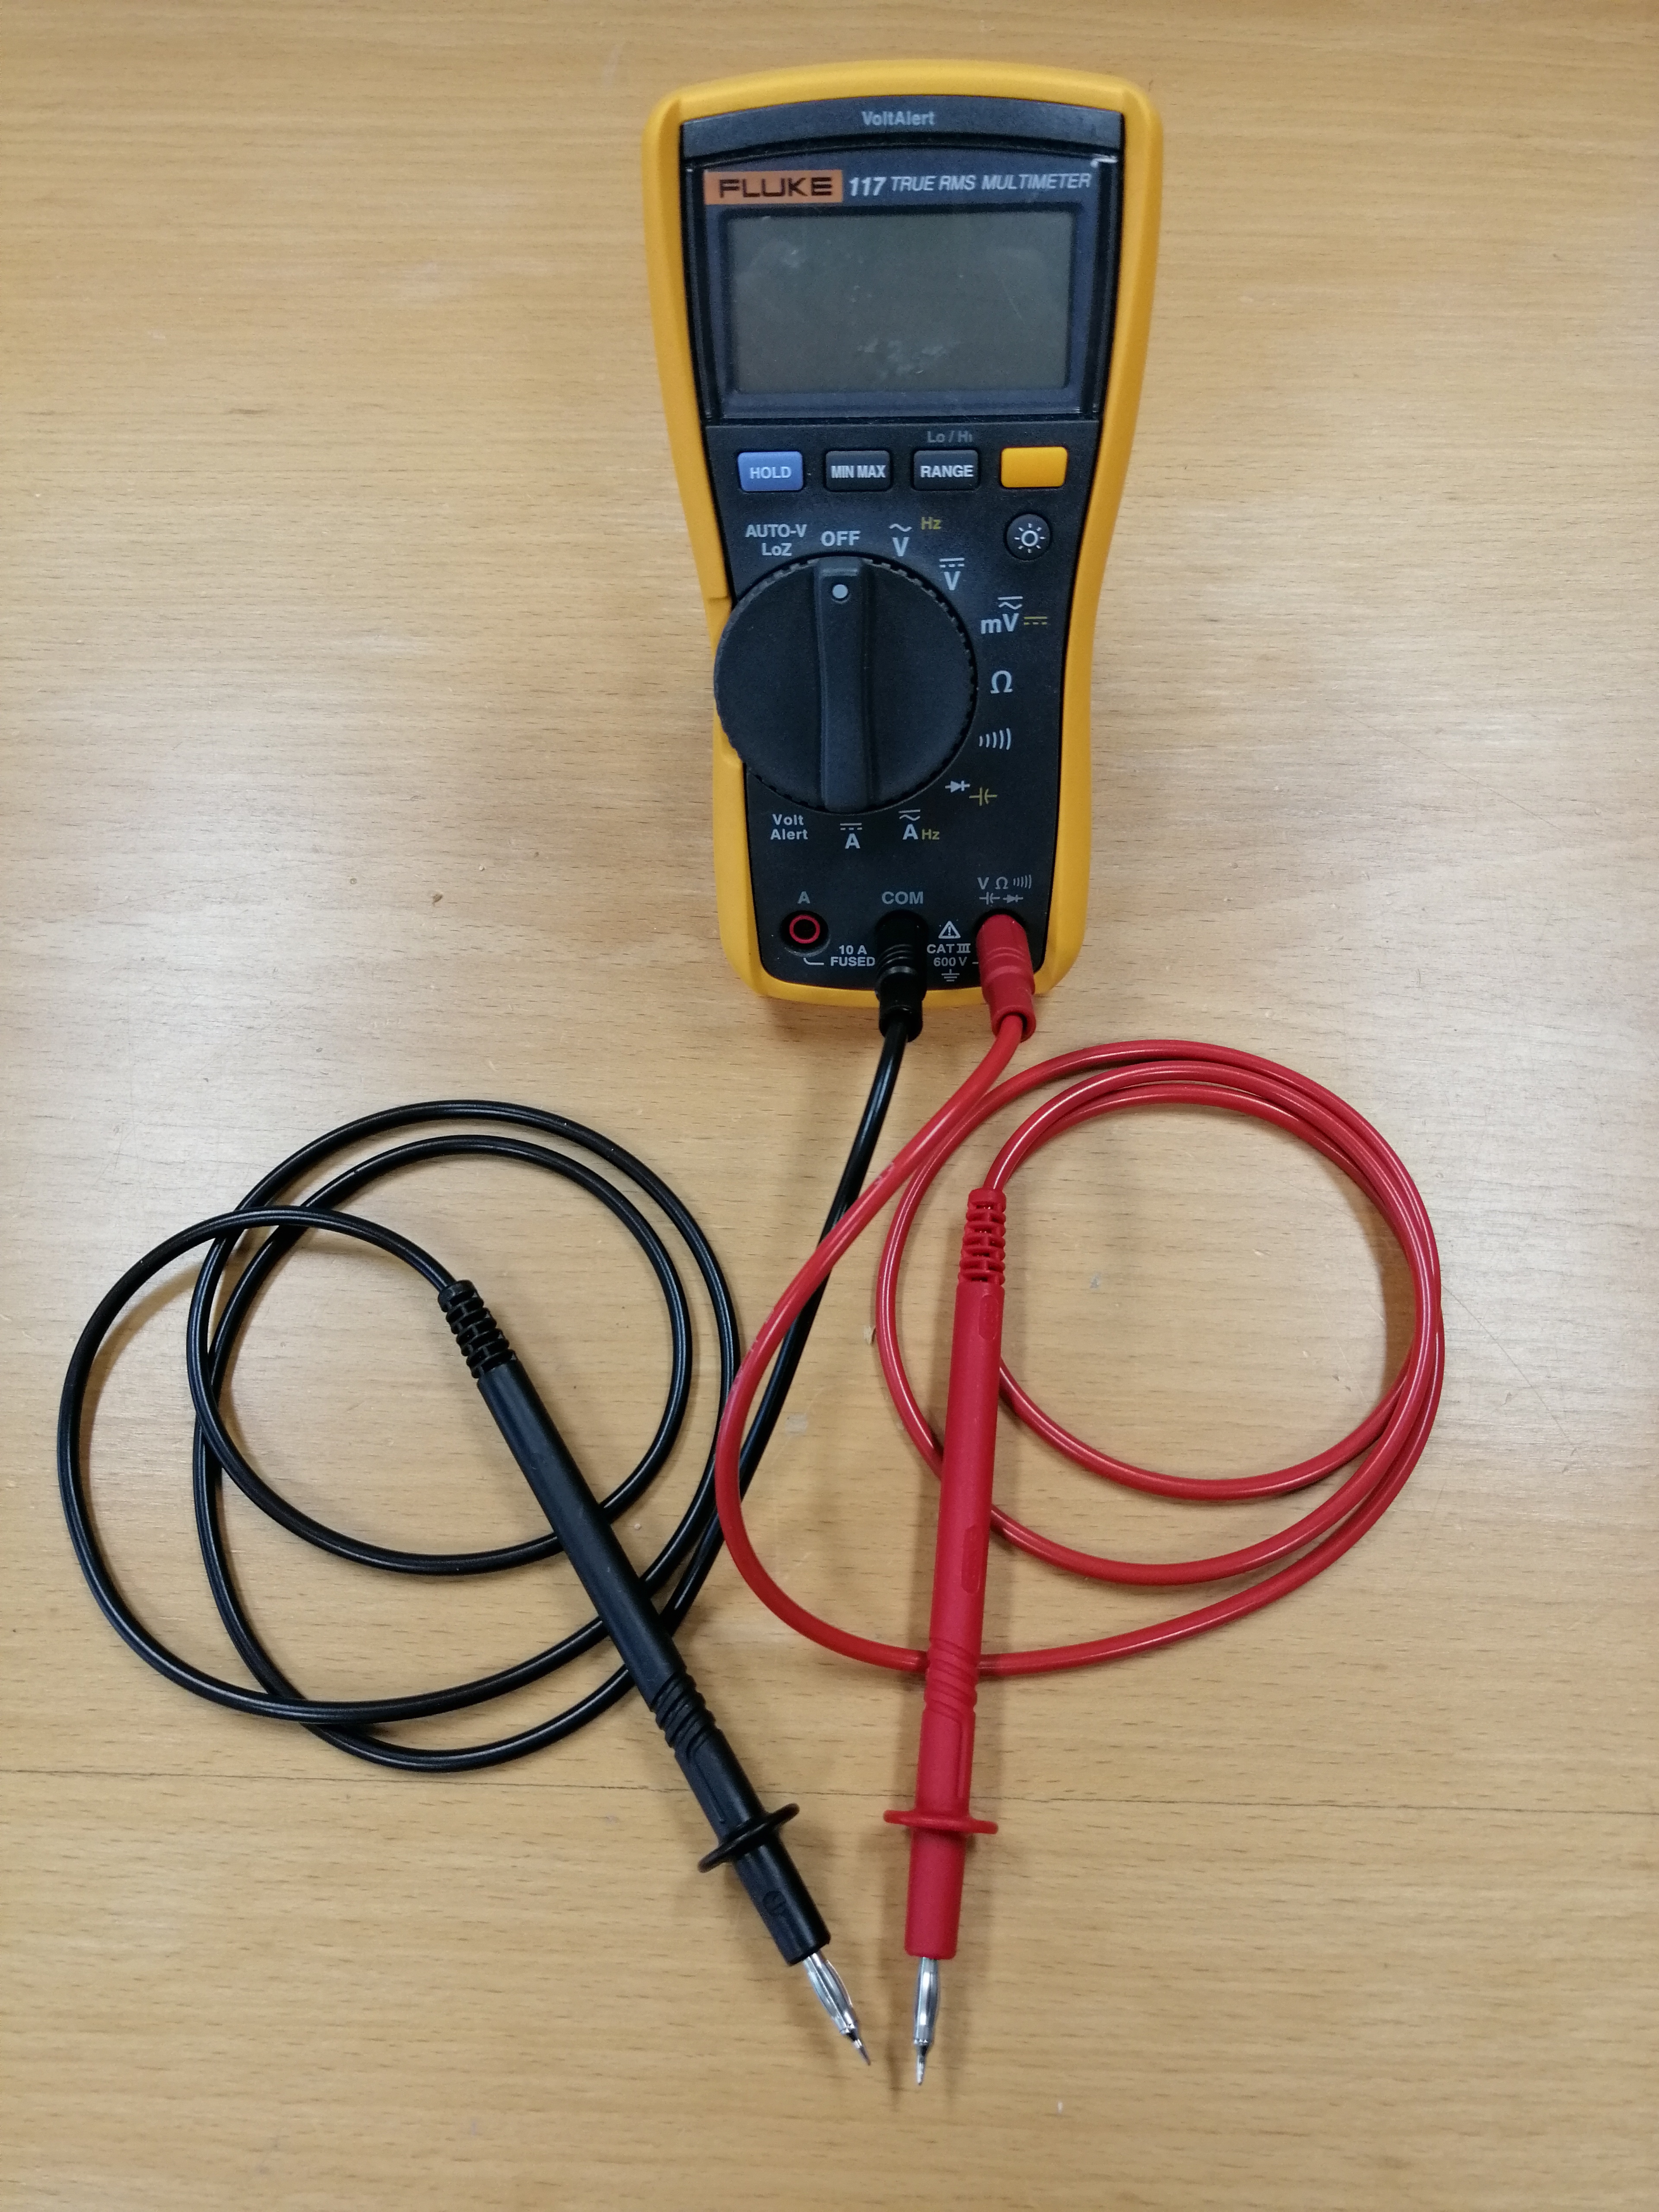
\includegraphics[width=0.6\linewidth]{graphics/HW_Val/Fluke.jpg}
\captionof{figure}{Das handliche RMS Multimeter FLUKE 117 mit Sonden.}
\label{fig:FLUKE}
\end{minipage}}

{\begin{minipage}[b][7cm][t]{0.49\textwidth}
\centering
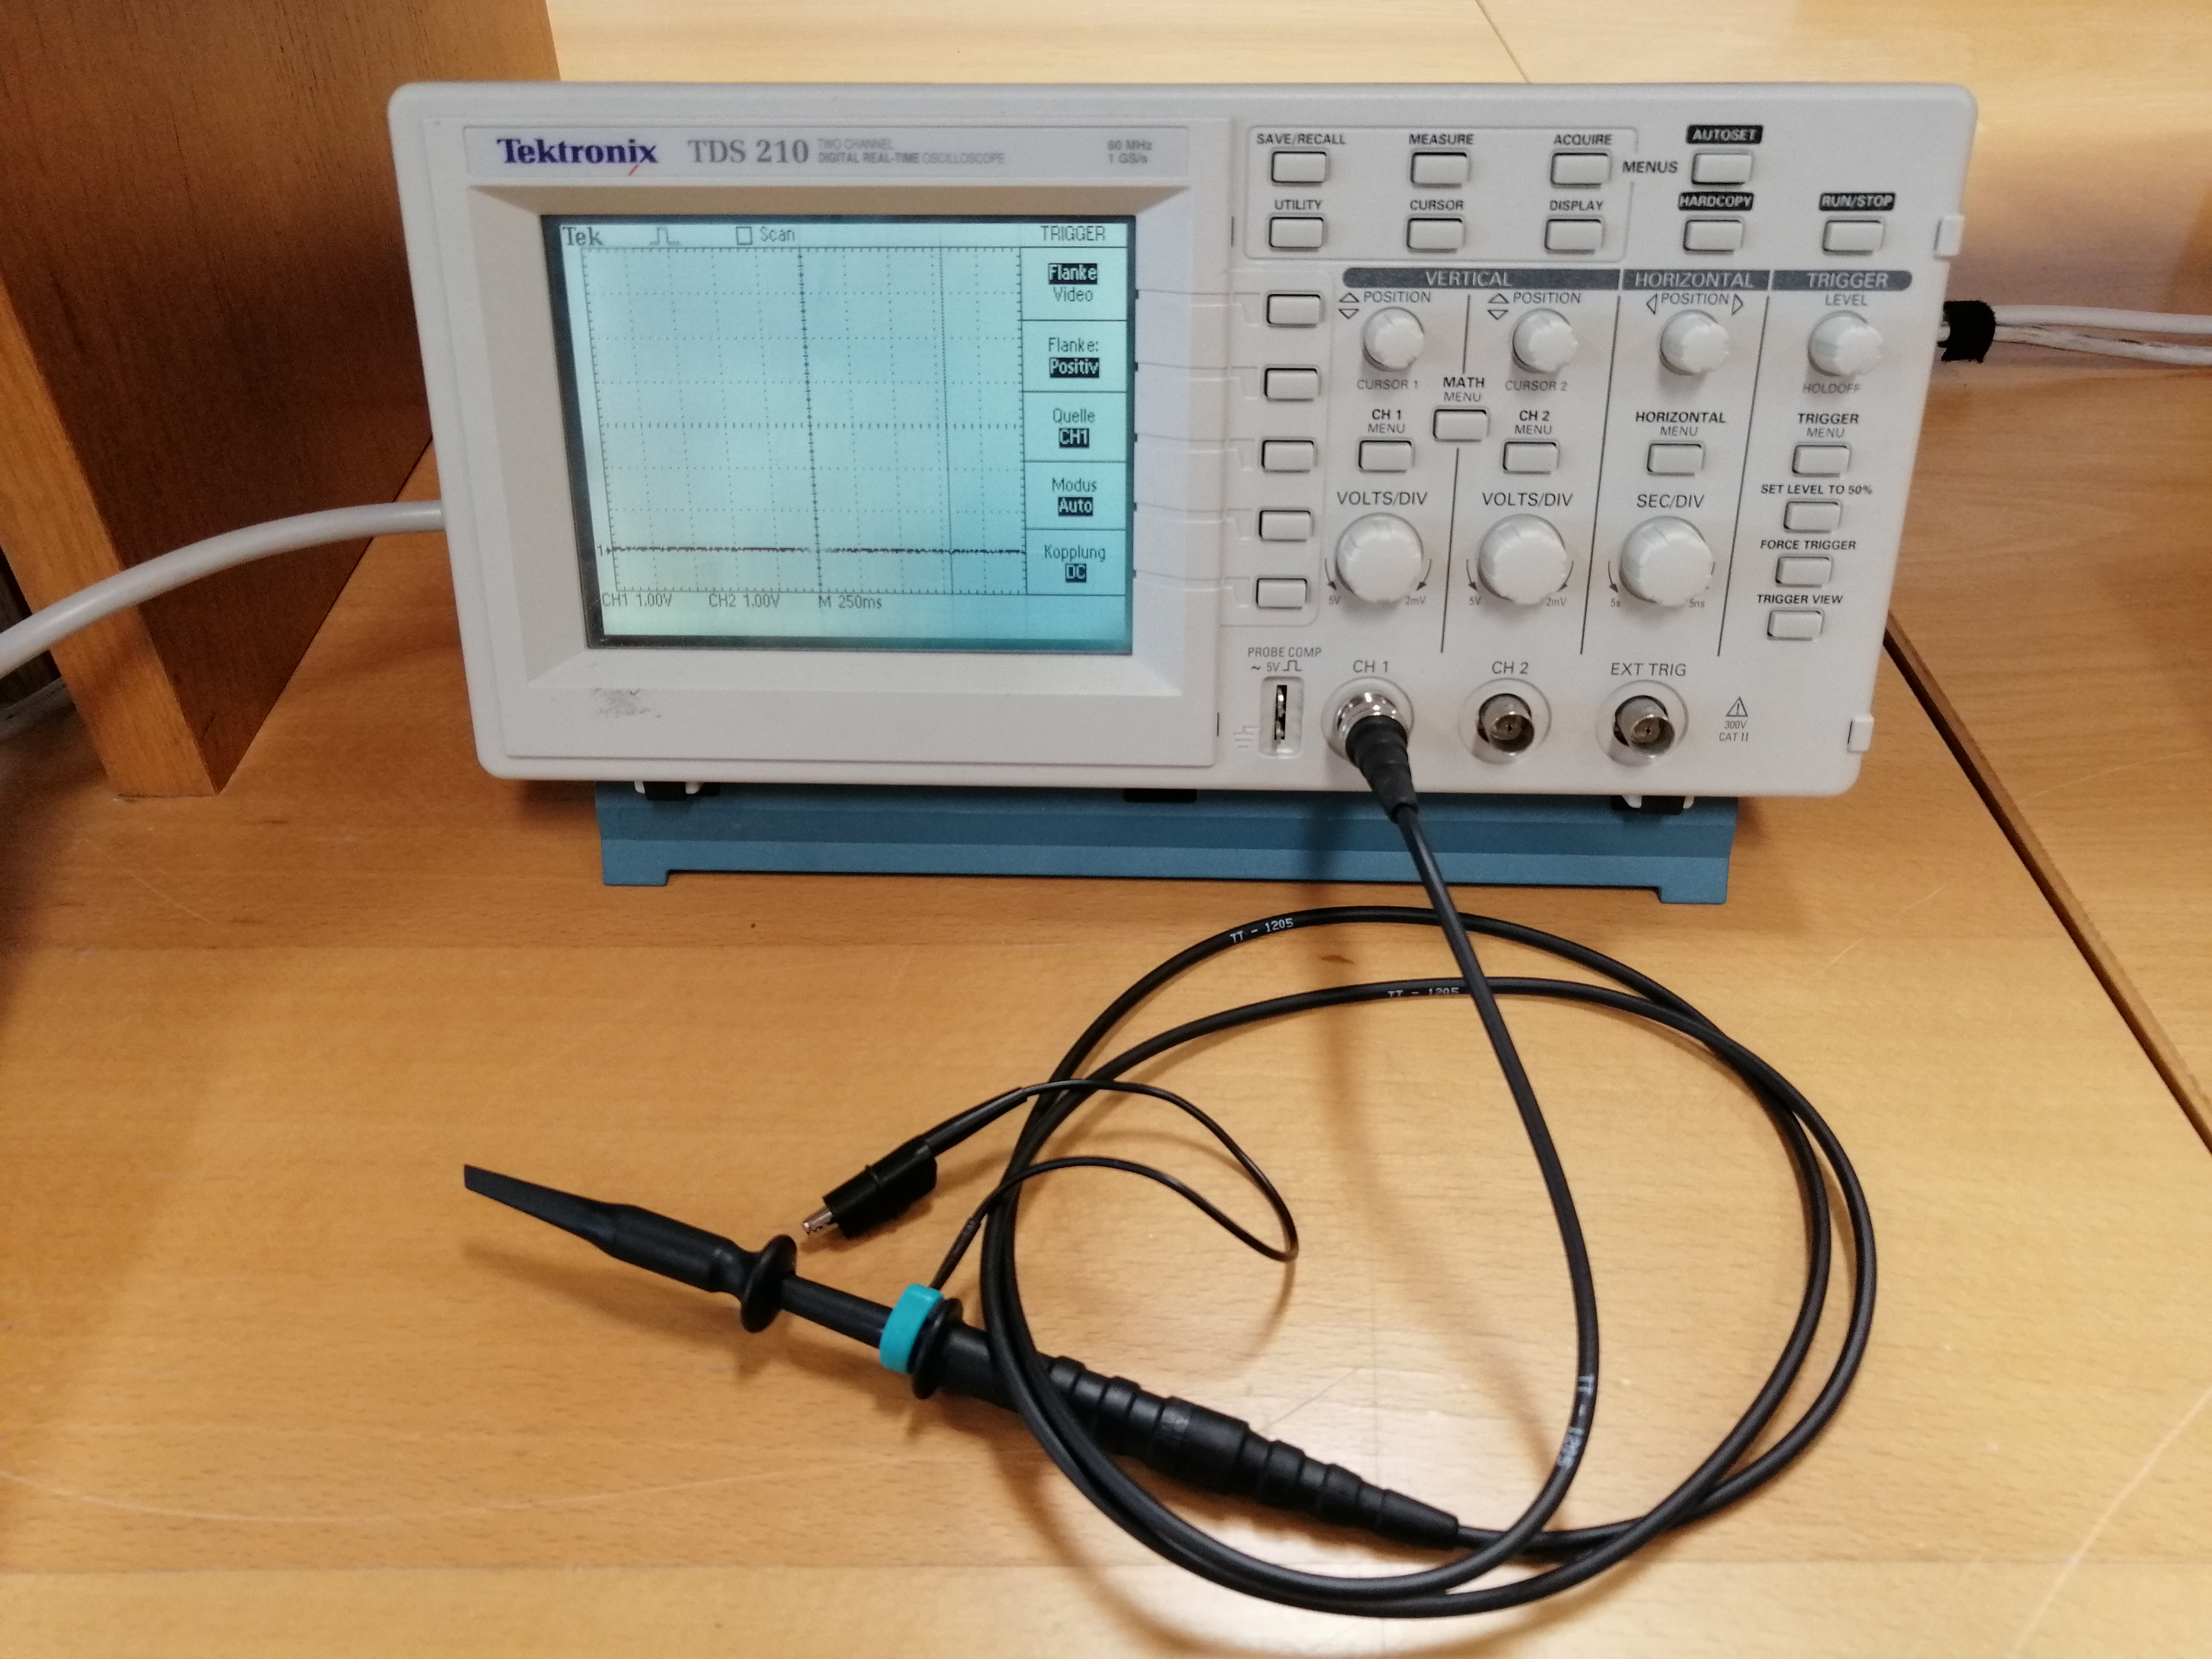
\includegraphics[width=0.9\linewidth]{graphics/HW_Val/KO.jpg}
\captionof{figure}{TDS 210 von Tektronix.}
\label{fig:KO}
\end{minipage}}
{\begin{minipage}[b][7cm][t]{0.49\textwidth}
\centering
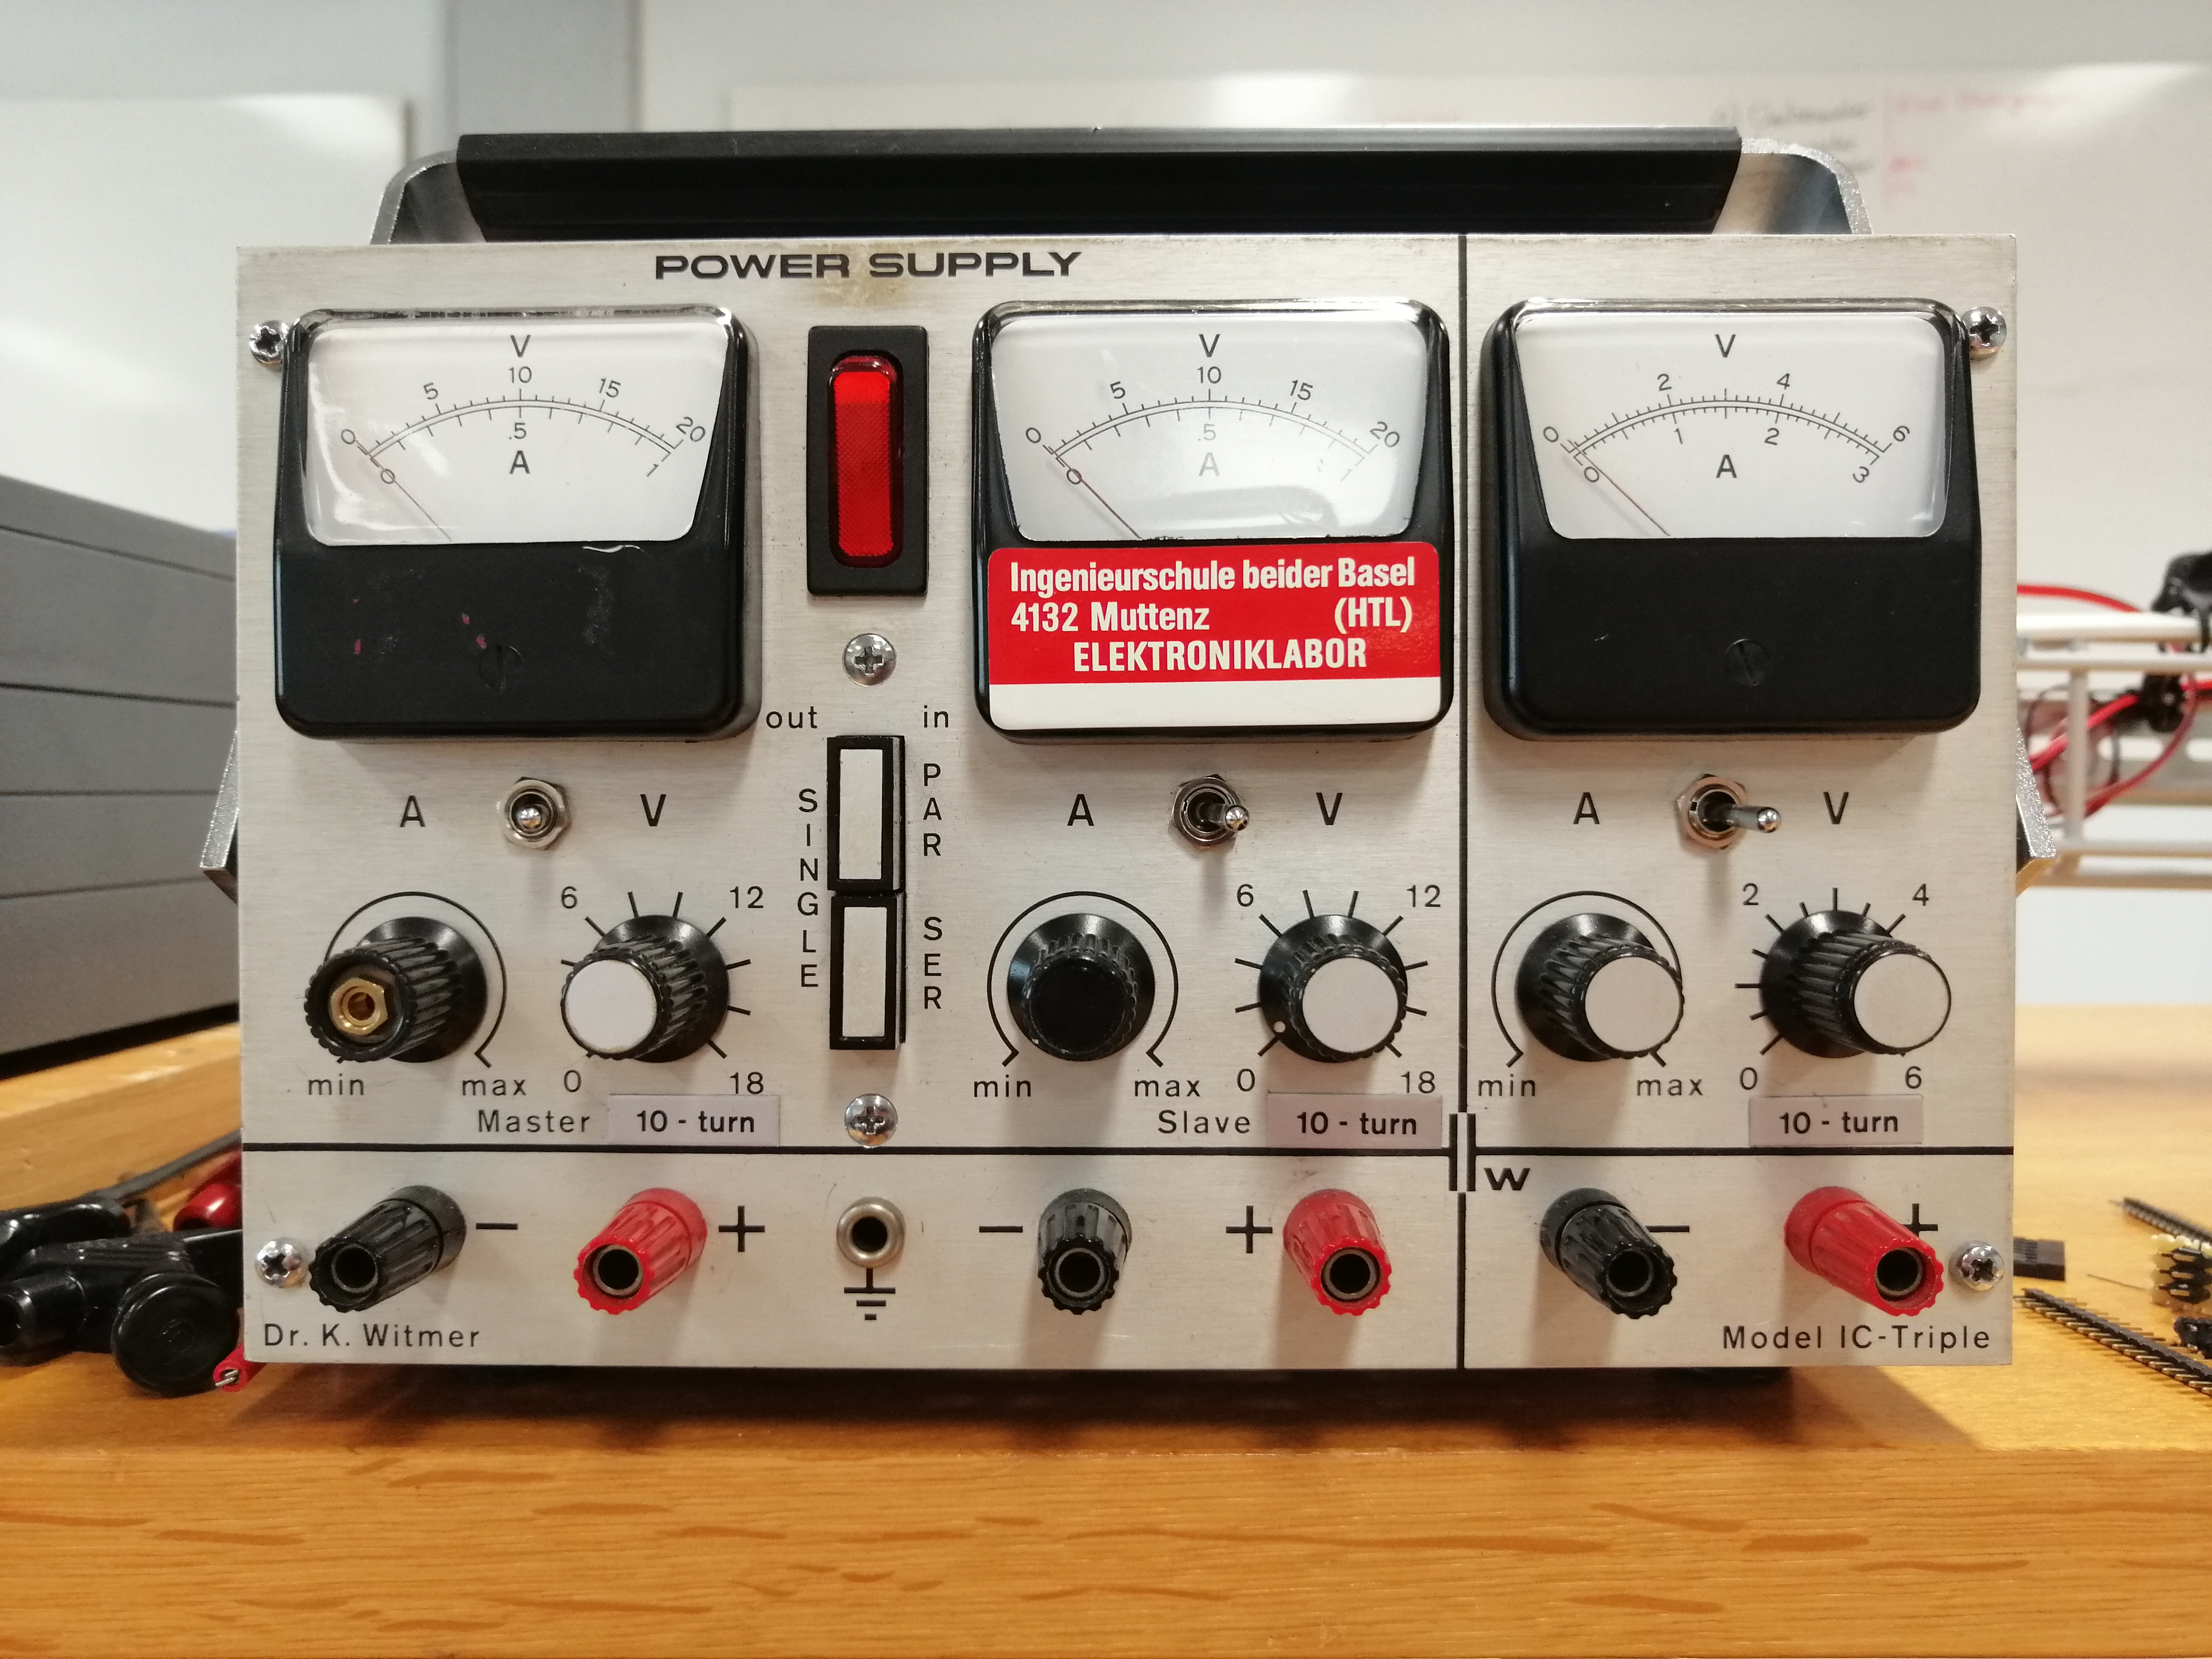
\includegraphics[width=0.9\linewidth]{graphics/HW_Val/PowerSupply.jpg}
\captionof{figure}{Das verwendete Speisegerät.}
\label{fig:PowerSupply}
\end{minipage}}

Die Geräte wurden nun vorgestellt, weshalb im nächsten Abschnitt bereits mit der Validierung der Energieversorgung begonnen wird.
\newpage
\paragraph{\textbf{Validierung der Energieversorgung}}[0.4cm]
{\begin{minipage}[b][6.5cm][t]{0.42\textwidth}
Die Energieversorgung ist äusserst wichtig, da ohne eine funktionierende Energieversorgung kein Bauteil seiner Funktion nachgehen kann. Zuerst wird kontrolliert, ob die Verbindungen der Leiterbahnen für das 3.3V-Netz bestehen. Dies wird mit der Kontinuitätsfunktion (Abbildung \ref{fig:Kontinuitaet}) des Flukes gemacht, bei welcher ein Ton erklingt sobald eine elektrische Verbindung besteht (kleiner Widerstand). Es werden vom Ausgang des Linearreglers aus alle Verbindungen getestet, welche in Abbildung \ref{fig:Verbindungstestpunkte} eingezeichnet wurden.
\end{minipage}}
{\begin{minipage}[b][6.5cm][t]{0.57\textwidth}
\centering
\includegraphics[width=0.6\linewidth]{graphics/HW_Val/Kontinuitaet.jpg}
\captionof{figure}{Das Zeichen für die Kontinuitätsfunktion des FLUKEs.}
\label{fig:Kontinuitaet}
\end{minipage}}
\begin{figure}[h]
\centering
\includegraphics[width=0.9\linewidth]{graphics/HW_Val/Verbindungstestpunkte.jpg}
\caption{Die Rot markierten Stellen zeigen die Endpunkte des Verbindungstests an. Die Orange markierte Stelle zeigt den Startpunkt an.}
\label{fig:Verbindungstestpunkte}
\end{figure}

Die Verbindungen konnten erfolgreich verifiziert werden. Bei jedem Punkt gemäss Abbildung \ref{fig:Verbindungstestpunkte} ist ein Signalton aus dem FLUKE gekommen, was eine bestehende elektrische Verbindung signalisiert.

Als zweites wird nach dem Bestücken der Energieversorgung diese ausgetestet. Es wird überprüft, ob der Linearregler am Ausgang auf 3.3V regelt. Ausserdem muss überprüft werden, ob die ChargePump die Akkuspannung auf das gewünschte Potenzial bringt. Darüber hinaus muss noch getestet werden, ob die Dioden in der nähe des DCIN Jacks wie gewünscht in Sperrichtung sperren. Für diese Tests müssen Spannungsverläufe auf dem TDS 210 betrachtet werden, sowie mit dem Speisegerät eine Eingangsspannung erzeugt werden. Die nachfolgende Bilder zeigen jeweils die Testpunkte der Messung, sowie die Visualisierung der gemessenen Spannung auf dem TDS 210.\\[0.5cm]

{\begin{minipage}[b][8cm][t]{0.49\textwidth}
\centering
\includegraphics[width=0.9\linewidth]{graphics/HW_Val/Test_Eingangsspannung.jpg}
\captionof{figure}{Testpunkt zur Überprüfung der Eingangsspannung.}
\label{fig:Test_Eingangsspannung}
\end{minipage}}
{\begin{minipage}[b][8cm][t]{0.49\textwidth}
\centering
\includegraphics[width=0.9\linewidth]{graphics/HW_Val/Ergebnis_Eingangsspannung.jpg}
\captionof{figure}{Die Eingangsspannung auf dem TDS 210 visualisiert. Es werden 4V angezeigt.}
\label{fig:Ergebnis_Eingangsspannung}
\end{minipage}}

{\begin{minipage}[b][8cm][t]{0.49\textwidth}
\centering
\includegraphics[width=0.9\linewidth]{graphics/HW_Val/Test_ChargePump.jpg}
\captionof{figure}{Testpunkt um die Spannungserhöhung der ChargePump zu messen.}
\label{fig:Test_ChargePump}
\end{minipage}}
{\begin{minipage}[b][8cm][t]{0.49\textwidth}
\centering
\includegraphics[width=0.9\linewidth]{graphics/HW_Val/Ergebnis_ChargePump.jpg}
\captionof{figure}{Die durch die ChargePump erhöhte Spannung, welche auf dem TDS 210 visualisiert wurde. Es werden etwas mehr als 6V angezeigt.}
\label{fig:Ergebnis_ChargePump}
\end{minipage}}

{\begin{minipage}[b][8cm][t]{0.49\textwidth}
\centering
\includegraphics[width=0.9\linewidth]{graphics/HW_Val/Test_Ausgangsspannung.jpg}
\captionof{figure}{Testpunkt für die Ausgangsspannung des Linearreglers.}
\label{fig:Test_Ausgangsspannung}
\end{minipage}}
{\begin{minipage}[b][8cm][t]{0.49\textwidth}
\centering
\includegraphics[width=0.9\linewidth]{graphics/HW_Val/Ergebnis_Ausgangsspannung.jpg}
\captionof{figure}{Die durch den Linearregler geregelte Ausgangsspannung. Es werden rund 3.3V angezeigt.}
\label{fig:Ergebnis_Ausgangsspannung}
\end{minipage}}

Die Abbildungen \ref{fig:Test_Eingangsspannung}, \ref{fig:Test_ChargePump} und \ref{fig:Test_Ausgangsspannung} zeigen die Testpunkte, an denen gemessen wurde. Die Ergebnisse davon sind in den Abbildungen \ref{fig:Ergebnis_Eingangsspannung}, \ref{fig:Ergebnis_ChargePump} und \ref{fig:Ergebnis_Ausgangsspannung} zu sehen. Das Ergebnis der Eingangsspannung zeigt, dass kein Kurzschluss vorhanden ist und die Spannung vom Speisegerät her auf dem PCB ankommt. Gemäss dem Ergebnis der Messung der ChargePump stellt man fest, dass diese ebenfalls funktioniert und die Spannung deutlich erhöht. Der Linearregler erzeugt aus der Spannung der ChargePump die benötigten 3.3V, was dem Ergebnis dieser Messung zu entnehmen ist. Es kann gesagt werden, dass die Energieversorgung soweit funktioniert.
\todo[inline]{Wie niedrige Spannung noch funktionstauglich, messung mit solarpanel ebenfalls}

Versorgungstechnisch hat das PCB die Tests bestanden, weshalb nun mit dem Herzstück der Wetterstation, der MCU-Bauteilgruppe, fortgefahren wird.

\paragraph{\textbf{Validierung der MCU-Bauteilgruppe}}[0.2cm]
In einem weiteren Schritt wird die MCU mit ihrer Peripherie auf dem PCB angelötet. Um zu testen, ob die MCU funktioniert, wird diese über den ICSP-Header geflasht (über ein AVR-Dragon) und dabei auf einen externen 8MHz-Clock eingestellt. Die LED soll nach dem flashen zu Testzwecken blinken, da die MCU in betrieb ist. Ausserdem soll die LED nicht mehr leuchten, solange der Reset-Button gedrückt wird.

{\begin{minipage}[b][8cm][t]{0.49\textwidth}
\centering
\includegraphics[width=0.9\linewidth]{graphics/HW_Val/MCU_flashen.jpg}
\captionof{figure}{Verbindung zwischen AVR-Dragon und MCU.}
\label{fig:MCU_flashen}
\end{minipage}}
{\begin{minipage}[b][8cm][t]{0.49\textwidth}
\centering
\includegraphics[width=0.9\linewidth]{graphics/HW_Val/MCU_LED.jpg}
\captionof{figure}{Die leuchtende LED der MCU.}
\label{fig:MCU_LED}
\end{minipage}}

{\begin{minipage}[b][7cm][t]{0.49\textwidth}
Abbildung \ref{fig:MCU_flashen} zeigt, wie die MCU mit einem Programm geflasht wird, wobei ein AVR-Dragon verwendet wird, welcher am ICSP Header angeschlossen ist. Das Blinken der LED kann leider nicht mit Bildern festgehalten werden, jedoch kann mit Hilfe des TDS 210 auch dieser Signalverlauf angezeigt werden, wie in Abbildung \ref{fig:Blinken_LED} ersichtlich.
\end{minipage}}
{\begin{minipage}[b][7cm][t]{0.49\textwidth}
\centering
\includegraphics[width=0.9\linewidth]{graphics/HW_Val/Blinken_LED.jpg}
\captionof{figure}{Signalverlauf der blinkenden LED.}
\label{fig:Blinken_LED}
\end{minipage}}

{\begin{minipage}[b][7cm][t]{0.49\textwidth}
\centering
\includegraphics[width=0.9\linewidth]{graphics/HW_Val/Testpunkt_Quarz.jpg}
\captionof{figure}{Messung am Quarz.}
\label{fig:Testpunkt_Quarz}
\end{minipage}}
{\begin{minipage}[b][7cm][t]{0.49\textwidth}
\centering
\includegraphics[width=0.9\linewidth]{graphics/HW_Val/Ergebnis_Quarz.jpg}
\captionof{figure}{Das oszillierende Signal des Quarzes auf dem TDS 210.}
\label{fig:Ergebnis_Quarz}
\end{minipage}}

An welcher Stelle der Quarz getestet wurde, ist in Abbildung \ref{fig:Testpunkt_Quarz} ersichtlich. Das Ergebnis kann in Abbildung \ref{fig:Ergebnis_Quarz} betrachtet werden. Es ist zu sehen, dass der Quarz mit den gewünschten 8MHz schwingt.

Da die MCU-Bauteilgruppe nun getestet wurde, wird als nächstes die serielle Schnittstelle ($\mu$USB-Anschluss) validiert, um weitere Bauteilgruppen mit dessen Hilfe validieren zu können.

\paragraph{\textbf{Validierung der seriellen Schnittstelle}}[0.2cm]
Die Bauteilgruppe der seriellen Schnittstelle wird nun auf dem PCB angelötet. Deren Funktion wird mit Hilfe eines Programms auf der MCU und PuTTY (ein Emulator für serielle Schnittstellen auf dem Computer) getestet.

{\begin{minipage}[b][7.5cm][t]{0.49\textwidth}
\centering
\includegraphics[width=0.9\linewidth]{graphics/HW_Val/Testpunkt_serial.jpg}
\captionof{figure}{Messung an einem Via der TRX-Signalbahn der MCU.}
\label{fig:Testpunkt_serial}
\end{minipage}}
{\begin{minipage}[b][7.5cm][t]{0.49\textwidth}
\centering
\includegraphics[width=0.9\linewidth]{graphics/HW_Val/Ergebnis_serial.jpg}
\captionof{figure}{Signalverlauf der von der MCU gesendeten Zeichen.}
\label{fig:Ergebnis_serial}
\end{minipage}}\\
Die Abbildungen \ref{fig:Testpunkt_serial} und \ref{fig:Ergebnis_serial} zeigen den Ort des gemessenen Signals und dessen Verlauf. Es ist ersichtlich, dass die gesendeten Zeichen von der MCU aus auf den FT231XS gelangen. Der Ausgang des FT231XS wird über die $\mu$USB-Schnittstelle an das Notebook gesendet und dort mit Hilfe von PuTTY auf dem Bildschirm sichtbar.

Daten können über die serielle Schnittstelle übertragen werden, womit im folgenden Abschnitt auf die Validierung der Datenspeicherung eingegangen werden kann.

\paragraph{\textbf{Validierung der Datenspeicherung}}[0.2cm]
Bei der Bauteilgruppe der Datenspeicherung wird mit Hilfe der seriellen Schnittstelle die Funktionsweise getestet. Dies geschieht, indem ein File auf der $\mu$SD-Karte gespeichert und über die serielle Schnittstelle ausgelesen wird.


Die Datenspeicherung wurde erfolgfreich validiert, weshalb im nächsten Abschnitt auf die etwas grössere Bauteilgruppe des SIM808 eingegangen wird.

\paragraph{\textbf{Validierung des SIM808}}[0.2cm]
Als nächster grosser Schritt wird die SIM808 mit deren Peripherie implementiert. Es wird getestet, ob die SIM-Karte eine 1.8V Speisung erhält (einfache Spannungsmessung). Nachfolgend wird dann das Senden und Empfangen einer SMS, sowie das ermitteln des Standorts über ein kleines Testprogramm getestet. Die LEDs werden dabei auf ihr korrektes Verhalten hin beobachtet. 

\todo[inline]{Fazit SIM808test}

Es wurden bereits einige Bauteilgruppen validiert, jedoch bleiben unter anderem die RTC, das Ombrometer, das Anemometer und der Windrichtungsgeber, weshalb im nächsten Abschnitt darauf eingegangen wird.

\paragraph{\textbf{Validierung der Peripherie und der RTC}}[0.2cm]
Nun werden die RTC, das Ombrometer und das Anemometer mit Windrichtungsgeber angeschlossen. Die Signale des Ombrometers, des Anemometers und des Windrichtungsgebers werden auf ein möglichst sauberes (unverrauschtes) Signal hin getestet und die Flanken des Ombrometers und des Anemometers auf Störungen untersucht. Die Flanke sollte gemäss Abbildung \ref{fig:Flankenbeispiel}, stetig steigend, aussehen, sodass keine Mehrfachdetektionen wegen Störungen auftreten.

\todo[inline]{Fazit RTC Anemo Ombro test}

Nun bleiben nur noch der BME280 und der TSL2561 offen für die Validierung, weshalb im nächsten Abschnitt darauf eingegangen wird.

\paragraph{\textbf{Validierung des BME280 und des TSL2561}}[0.2cm]
Zu guter letzt können der BME280 und der TSL2561 angeschlossen werden und über ein Testprogramm auf ihre korrekte Funktionsweise hin überprüft werden.

\todo[inline]{Fazit BME-TSL-test}

Die Hardware wurde validiert, es kann gesagt werden, dass alle Tests bestanden wurden. In einem weiteren Schritt muss nun die Firmware auf die MCU geladen und getestet werden, was im nächsten Kapitel erfolgt.